\documentclass[11pt]{article}
\usepackage[utf8]{inputenc}
\usepackage[T1]{fontenc}
\usepackage{amsmath}
\usepackage{amsfonts}
\usepackage{amssymb}
\usepackage[version=4]{mhchem}
\usepackage{stmaryrd}
\usepackage{graphicx}
\usepackage[export]{adjustbox}
\graphicspath{ {./images/} }

\begin{document}
Distressed Securities Funds

Distressed debt hedge funds invest in the securities of a corporation that is in bankruptcy or is likely to fall into bankruptcy. Companies can become distressed for any number of reasons, such as too much leverage on their balance sheet, poor operating performance, accounting irregularities, or even competitive pressure. Some of these strategies can overlap with private equity strategies. Distressed debt is discussed in detail in Session 4.5, Private Credit and Distressed Debt, since distressed debt is an important area of investment within private equity. The key difference is that private equity investors take a long-term view on the value and reorganization potential of the corporation, whereas hedge funds typically take a shorter-term trading view on distressed investments.

When evaluating investments across multiple layers of the capital structure, investors need to estimate the long-term value of each layer of the capital structure, which can be highly influenced by the priority of claims in a bankruptcy proceeding. The bankruptcy process is more fully covered in the session Private Credit and Distressed Debt on private equity; however, the following section covers material on the bankruptcy process that is essential to understanding distressed hedge fund strategies.

\section*{The Bankruptcy Process}
When the face value of the liabilities of a firm exceeds the market value of its assets, the bankruptcy process allocates the assets across various security holders and stakeholders of the firm. The bankruptcy process is the series of actions taken from the filing for bankruptcy through its resolution. Those who are paid after the most senior claims such as wages are paid are the holders of senior, secured, and collateralized debt. Once these senior claims have been satisfied, junior, subordinated, and convertible bondholders are next in line. In many cases, these junior debt holders do not receive a full recovery during the bankruptcy proceedings but may receive equity in the firm if it is reorganized. Last in line come preferred stock and equity holders in the firm, who often receive little or no value during the bankruptcy reorganization process.

In the United States, firms declaring bankruptcy may either liquidate or reorganize operations, but European firms typically face liquidation when they are deemed unable to meet their debt obligations. In a liquidation process (Chapter 7 in US bankruptcy laws), all of the assets of the firm are sold and the cash proceeds are distributed to creditors. A firm is liquidated when it is viewed as not viable as an ongoing entity. Firms with liquidity problems but with reasonable chances of being viable are reorganized. In a reorganization process (Chapter 11 in US bankruptcy laws), the firm's activities are preserved. The goal of a reorganization process is to stabilize the operations and finances of the company in a way that allows the firm to continue operations after the bankruptcy process has been completed. To strengthen the firm, contracts such as labor union contracts, pension programs, and real estate leases can be substantially revised during the process. Debt holders may agree to lengthen maturities, reduce coupon rates, or accept equity in the reorganized firm as a way of reducing the emerging company's cash outflows and debt burdens. During the reorganization process, the equity in the pre-bankrupt firm is typically canceled and becomes worthless as shares in the newly reorganized firm are either offered to subordinated debt holders or sold to new investors.

Distressed securities investments can be inefficiently priced and require active management. Positions in investment-grade equities require almost no ongoing involvement other than periodic voting. However, management of positions in distressed securities may require frequent participation in the bankruptcy process to negotiate and litigate better outcomes. Most distressed securities investments are one-off transactions. A one-off transaction has one or more unique characteristics that cause the transaction to require specialized skill, knowledge, or effort. Investors in traditional equity positions may rely to some extent on the availability of public information and the high level of competition in financial markets to drive market prices toward reflecting available information, meaning that the prices are informationally efficient. As securities involving unique situations, rapidly changing situations, information asymmetries, and limited numbers of institutional owners, distressed securities are less likely to trade at informationally efficient prices. Information asymmetries occur when individual economic actors possess different knowledge.

Thus, investing in distressed securities requires specialized, skillful, and ongoing analysis and involvement. Therein lies the potential of the strategy both to generate alpha and to contribute risk to the investor. However, seeking alpha through distressed investing does not necessarily mean involvement in an asset type that is a zero-sum game, wherein each investor with a positive alpha must be balanced by an investor with a negative alpha. Most institutions either do not want to directly invest in distressed securities or are unable to invest in distressed securities. Many institutions, such as insurance companies and pension funds, are prevented through regulation from purchasing or even holding substantial quantities of non-investment-grade securities. Other institutions may divest speculative holdings prior to bankruptcy for the following reasons: (1) to avoid the increased monitoring needs; (2) to avoid ending up with inappropriate securities (e.g., bond funds that might receive equity in the reorganization process); or (3) to avoid revelation of embarrassing investment holdings in future portfolio disclosures, meaning to window-dress the public view of the portfolio. It is argued that the dumping of securities by institutions as they spiral downward in quality causes low price levels that permit generous alphas to those providing liquidity to the market by purchasing the unwanted securities. Overall positive average alphas to distressed securities investing may therefore be generated by institutional factors and offered to distressed investors as a reward for the provision of liquidity.

\section*{Short Sales of Equity as Writing Naked Call Options}
There are many variations on how a hedge fund plays a distressed situation. The declaration of bankruptcy by a firm can vary from being made by viable firms seeking temporary protection from cash flow problems to highly distressed firms with virtually no chance of survival. When a firm known to be in financial trouble seeks bankruptcy protection and reorganization (Chapter 11 in the United States), the stock price often rises in recognition of the firm's decision to use the technique to solve its financial problems. However, surprise bankruptcy filings and Chapter 7 (liquidation) bankruptcy filings usually cause share price declines. Most of the following discussion focuses on firms for which bankruptcy is perceived to be likely to end in liquidation.

Prior to a bankruptcy, if an analyst views a situation as likely to deteriorate financially, the simplest trade is to sell short the stock of the distressed firm. This requires the hedge fund manager to borrow stock from its prime broker and sell the stock with the expectation that it will be able to purchase the stock back at a lower price in the future after the fundamentals of the firm have deteriorated. This is an unhedged speculation and nothing more than an attempt to sell high and buy low.

Short selling of a distressed company exposes the hedge fund manager to substantial risk if the company's fortunes suddenly improve. Perhaps the riskiest trade in the equity market is to be short the stock of a firm that is rumored to be descending into bankruptcy but recovers vigorously. Consider the stock of American Airlines, which traded below $\$ 2$ in March 2003, shortly after both United Airlines and US Airways declared bankruptcy. Similarly, shares of Ford traded below $\$ 2$ in November 2008 as General Motors approached bankruptcy. Unfortunately for short sellers, the shares of each firm traded above $\$ 11$ one year later, when it became clear that neither American Airlines nor Ford would declare bankruptcy anytime soon.

As is detailed in Topic 6 on structured products, shares in highly leveraged firms resemble call options. Short selling distressed equities is therefore analogous to writing naked call options on the firm's assets and generates a negatively skewed return distribution. An investor has a naked option position when the investor is short an option position for which the investor does not also have a hedged position, such as owning the underlying asset when short a call and being short the underlying asset when short a put. The negative skew is seen in the previous examples in the potential gain of $\$ 2$ and potential loss of $\$ 9$ or more in the shares of American Airlines and Ford. Conversely, an analyst who views share prices as reflecting overestimated probabilities of further deterioration in the firm's financial condition may establish long positions in the firm's equity and typically receive a positively skewed return distribution.

After most bankruptcy filings, the stocks are delisted. In some cases, there is almost no probability that the firm will distribute any cash to equity holders, and therefore the stocks are virtually worthless. Nevertheless, it is sometimes the case that the shares trade at values that reflect unrealistic probabilities of survival. Some investors are comfortable selling short shares in companies after bankruptcy is declared, even at prices of $\$ 0.50$ per share or less. However, a caveat must be provided regarding the potential danger. Shares of USG Corporation (USG) and General Growth Properties (GGP) rallied sharply while in bankruptcy. USG shares, which traded below $\$ 3$ in 2002, rallied to over $\$ 110$ per share early in 2006 before exiting bankruptcy. Similarly, GGP shares, which traded below $\$ 0.20$ in late 2008 , increased in value to over $\$ 15$ by the end of 2010 , as it became clear that the value of the firm's real estate holdings exceeded the outstanding value of the debt.

\section*{Searching for Distressed Undervalued Securities and Estimating Recovery Value}
The prices of debt in distressed firms can trade substantially below face value before and during the bankruptcy process. Senior debt typically has higher prices than subordinated debt of the same firm due to the higher priority of claims on the assets of the firm. At the time of the bankruptcy filing, many debt holders sell their bonds due to restrictions on the credit quality of holdings that may be imposed by insurance or pension plan regulators or simply because of investors' unwillingness to stomach the risk or tolerate the time-intensive nature of holding and evaluating distressed securities. In cases of poor market liquidity, debt securities of these firms may be undervalued and therefore offer return from alpha in addition to a systematic risk premium for their market risks.

The job of a distressed investor sounds simple: Estimate the recovery value. The recovery value of the firm and its securities is the value of each security in the firm and is based on the time it will take the firm to emerge from the bankruptcy process and the condition in which it will emerge. Unfortunately, analyzing probabilities and outcomes and making both of these estimations can be difficult and firm-specific processes. The estimated liquidation or reorganized value of assets is analyzed with the priority of claims to arrive at the estimated recovery rates for each bond issue. The recovery rate of a bond is the portion of face value that is ultimately received by an investor in a bond issue at the end of the bankruptcy proceedings. Securities with higher seniority in bankruptcy generally experience higher recovery rates and are therefore worth more than junior securities. Thus, a firm may have senior debt issues trading at $60 \%$ of par value and subordinated debt issues trading at $30 \%$ of par value, even though they share the same underlying assets.

The recovery value of distressed securities at liquidation can be especially sensitive to market conditions in the industry. Consider the bankruptcy of an electric utility such as Enron. When the firm is liquidated, hard assets, such as power plants, need to be sold in a relatively short time frame. When the entire industry is in distress and overleveraged, it may be necessary to sell these assets at depressed prices. Some distressed investors-especially when the firm will need to sell substantial industry-specific assets-hedge the recovery rate risk by selling short shares in firms that have similar assets.

The time that firms spend in bankruptcy can vary widely, even when the firms are of relatively similar size and from the same industry. For example, US Airways spent just seven months in bankruptcy court, from August 2002 to March 2003, but United Airlines spent over three years, from December 2002 to February 2006, finally reemerging as a reorganized firm.

\section*{Estimating Returns from Undervalued Securities}
The annualized returns of deals involving distressed investing are highly influenced by the time the company spends under the supervision of the bankruptcy court. For example, consider an investor who buys a senior debt issue at $60 \%$ of face value and a subordinated debt issue at $30 \%$ of face value that yield eventual recovery values of $80 \%$ and $50 \%$, respectively. These recovery values would generate non-annualized returns of $33.3 \%$ on the senior debt and $66.7 \%$ on the subordinated debt, assuming no coupon income. These returns are computed as the difference in the percentage of face value invested relative to the percentage of face value recovered, expressed as a percentage of the invested quantity. In the example of a six-month bankruptcy process, these returns represent annualized returns of $67 \%$ $(33.33 \% \times 2)$ on the senior debt and $133 \%(66.7 \% \times 2)$ on the subordinated debt, ignoring compounding. But for a deal that takes 3.33 years to work out, the same deal generates annualized returns of $10 \%$ on the senior debt and $20 \%$ on the subordinated debt, ignoring compounding.

Investors may also profit from determining if and when the company will declare bankruptcy. An understanding of the financial condition of the firm based on financial statements and other information is key, as the investor needs to estimate how cash flows, including interest expense and debt maturities, can affect the timing of the bankruptcy. An investor who predicts that a bankruptcy filing will not occur for two years, perhaps a longer view than the market's, can profit if correct by buying debt issues with less than two years until maturity while selling short debt issues with more than two years until maturity. If the first debt issue is repaid at its full face value before the company files for bankruptcy and before the maturity of the later debt issue, the distressed investor has probably earned alpha.

\section*{Distressed Activists}
Many distressed investors do not take an activist approach; rather, they simply buy distressed securities and wait for the events related to reorganization to unfold. Activist investors in distressed securities seek to influence both the recovery value and the timing of the exit from the bankruptcy process. The activist approach is an intense process that requires a substantial amount of legal work as the manager negotiates with the court and other investors.

The activist investor may simply choose to expedite the bankruptcy process by cooperating with other parties, which may lower ultimate recovery rates but increase annualized returns. Alternatively, the activist may attempt to improve its position relative to other parties in the priority of claims with a less cooperative approach that may generate higher recovery values as well as delays in distributions.

\section*{Capital Structure Arbitrage}
Unhedged positions in distressed firms, such as simple long positions or short positions in equity or other securities, involve relatively high risk. Unhedged positions in distressed securities are plays on absolute value and are subject to substantial idiosyncratic and systematic risks. Most hedge fund managers typically use a hedging strategy known as capital structure arbitrage. Capital structure arbitrage involves offsetting positions within a company's capital structure with the goal of being long relatively underpriced securities, being short overpriced securities, and being hedged against risk. These hedged positions have reduced exposure to the general risks of the economy or the firm and are plays on relative values within the firm's capital structure.

For a traditional capital structure arbitrage trade, investors typically buy the more senior claim and sell short the more junior claim. Consider a company that has four levels of outstanding capital: senior secured debt, junior subordinated debt, preferred stock, and common stock. Two standard distressed security investment strategies are (1) to buy the senior secured debt and short the junior subordinated debt, or (2) to buy the preferred stock and short the common stock.

In a bankruptcy, the senior secured debt stands in line in front of the junior subordinated debt for any bankruptcy-determined payouts. The same is true for the preferred stock compared to the common stock. In both of the common capital structure arbitrage strategies just detailed, there is a long position in the more senior security and a short position in the more junior security for each pair. Therefore, in both cases, the strategy is long the security with the higher standing in the bankruptcy process.

Consider the case of buying the senior secured debt and shorting the junior subordinated debt. Assume that equal dollar positions of $\$ 10,000$ (of opposite sign) are established in both bonds at discounts to face value, with the senior debt trading at a smaller discount than the junior debt. The gains and losses on this hedged position depend on the relative movements of the constituent positions. There are four cases that provide insight into the risks of this traditional hedge:

\begin{enumerate}
  \item At the bearish extreme for the firm's assets, no recovery is ever received on either bond, and the hedge breaks even by gaining $\$ 10,000$ on the short position and losing $\$ 10,000$ on the long position.

  \item On the bullish extreme for the underlying assets, full recovery is made on both bonds, and the loss on the short exceeds the gain on the long, causing the hedge to lose money.

  \item If the senior debt is fully recovered and the junior debt has no recovery, the hedged position gains on both legs of the trade and generates a large profit.

  \item If recovery rates of the bonds are equal, the junior bond gains more and the hedge generates a net loss.

\end{enumerate}

Thus, capital structure arbitrage is not a simple bullish or bearish bet on the eventual value of the firm's assets that can be distributed to security holders. The key to traditional capital structure arbitrage profitability is when the more senior security improves more, or deteriorates less, than the junior security. Note that the analysis assumed equal sizes for the long and short positions. Other hedge ratios are common, and they can generate substantially different profits and losses for various outcomes.

Senior claims in distressed debt securities tend to offer higher loss potential and lower profit potential than do junior claims. For example, the equity can resemble a call option or a lottery ticket, with a small investment required and a small chance of a large payout. If less sophisticated investors prefer the return distributions of the junior claims, it is possible that more sophisticated investors can consistently profit from the traditional capital structure arbitrage strategies to the extent that the market overprices the more junior claims and underprices the more senior claims.

Derivative securities can expand the opportunities available for capital structure arbitrage and make strategies more versatile and riskier. In some cases, especially pre-bankruptcy, it is argued that financial market segmentation occurs such that the stock market and the bond market may be valuing securities based on very different appraisals of the firm's prospects. Financial market segmentation occurs when two or more markets use different valuations for similar assets due to the lack of participants who trade in both markets or who perform arbitrage between the markets. The idea is that each market attracts its own clientele, and the different clienteles generate different values.

For example, the bonds of General Motors (GM) were rated as CCC at a time when GM stock was trading at over $\$ 20$ per share. Assuming that these observations indicated sharply divergent valuation standards in the debt and equity markets, investors could have chosen to perform capital structure arbitrage with the legs of the trade in different markets. A hedge fund manager could have bought put options on GM stock to hedge a long position in GM bonds. Derivatives expand the set of markets pricing a deal by adding derivative markets. Thus, a capital structure arbitrage opportunity may be designed to exploit perceived mispricing due to financial market segmentation. The CDS market is also a key component of capital structure arbitrage strategies, providing cost-effective vehicles for hedging credit risk in long or short positions in corporate debt. CDS protection is bought and sold in the over-the-counter market, further increasing opportunities to exploit financial market segmentation.

\section*{Buying the Firm Using Distressed Securities}
A distressed securities hedge fund can become involved in the bankruptcy process as a strategy for establishing a controlling position in firms that the fund perceives as substantially undervalued. This is where an overlap with the strategies of private equity firms can occur. To the extent that a distressed securities hedge fund is willing to learn the arcane workings of the bankruptcy process and participate in its steps, including sitting on creditor committees, substantial value can be realized if the distressed company can be successfully restructured and is able to regain its profitability. This strategy, with its intention of gaining a controlling interest, differs from that of hedge fund managers who purchase the securities of a distressed company shortly before it announces its reorganization plan to the bankruptcy court. The latter case is based on the expectation of a positive resolution with the company's creditors, whereas the former case includes a desire to obtain control.

\section*{Key Observations Regarding Historical Returns of Distressed Funds}
Monthly returns to distressed funds are observed from January of 2000 to December of 2021 for a total of 264 observations. Statistical Summary of Returns provides univariate return statistics and partial autocorrelations of returns in the top panel, and a histogram of returns in the bottom panel.

\begin{center}
\begin{tabular}{lcc}
\hline
\begin{tabular}{c}
Index (Jan. 2000- \\
Dec. 2021) \\
\end{tabular} & \begin{tabular}{c}
HFRI Event-Driven: Distressed \\
/Restructuring Index \\
\end{tabular} & \begin{tabular}{c}
MSCI World \\
Equity \\
\end{tabular} \\
\hline
Annualized Arithmetic Mean & $7.4 \%$ & $6.8 \%$ \\
Annualized Standard Deviation & $6.6 \%$ & $15.4 \%$ \\
Annualized Semivolatility & $5.8 \%$ & $11.8 \%$ \\
Annualized Median & $9.4 \%$ & $15.1 \%$ \\
Skewness & -1.4 & -0.6 \\
Excess Kurtosis & 6.9 & 1.6 \\
Sharpe Ratio & 0.7 & 0.3 \\
Sortino Ratio & 0.8 & 0.4 \\
Annualized Geometric mean & $7.1 \%$ & $5.6 \%$ \\
First-Order Autocorrelation & 0.4 & 0.1 \\
Annualized Standard Deviation & $10.3 \%$ & $17.0 \%$ \\
(Adjusted for Autocorrelation) & $6.4 \%$ & $12.8 \%$ \\
Maximum & $-11.1 \%$ & $-19.0 \%$ \\
Minimum & $-27.4 \%$ & $-54.0 \%$ \\
Max Drawdown &  &  \\
\end{tabular}
\end{center}

\begin{center}
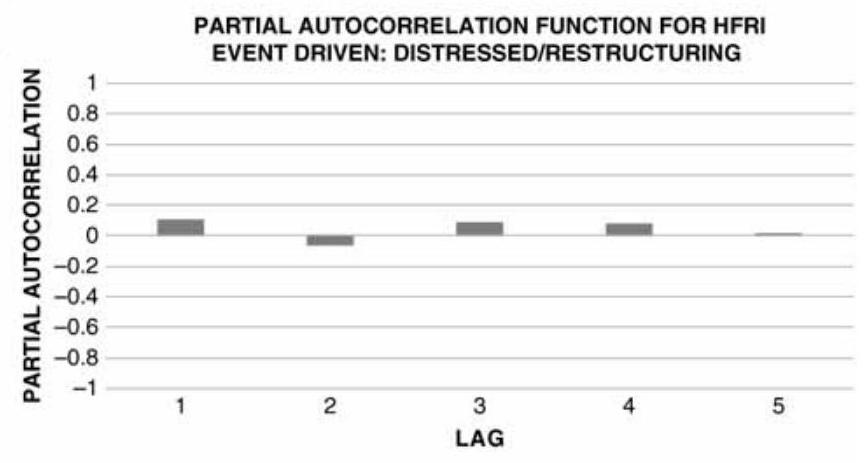
\includegraphics[max width=\textwidth]{2024_04_09_96054006c4d1a1e0ab8bg-5}
\end{center}

Histogram of HFRI Event Driven: Distressed/Restructuring Returns (Monthly) Jan. 2000-Dec. 2021

\begin{center}
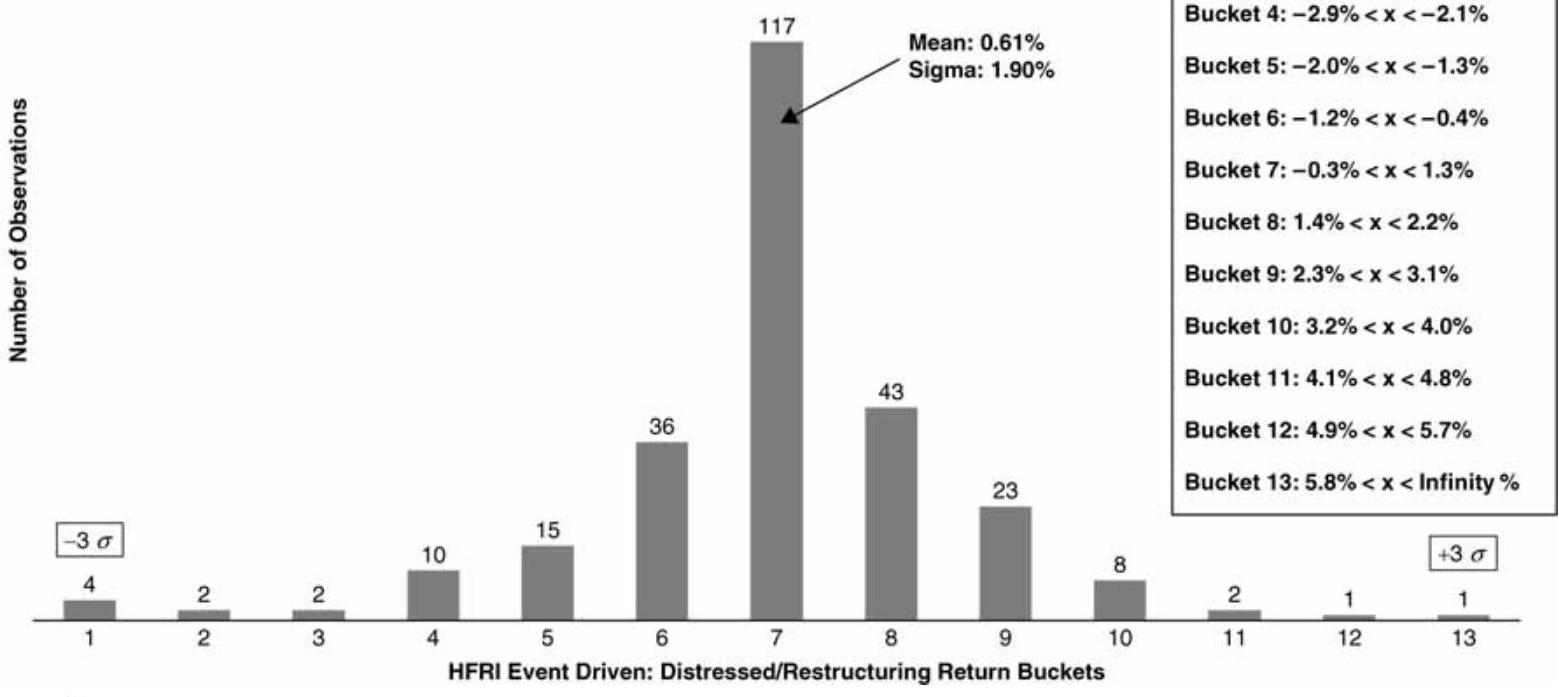
\includegraphics[max width=\textwidth]{2024_04_09_96054006c4d1a1e0ab8bg-5(1)}
\end{center}

\section*{Statistical Summary of Returns}
Key observations on the returns to distressed funds that are consistent with economic reasoning are an essential component of knowledge and include the following:

\begin{enumerate}
  \item Event-driven distressed returns exhibited substantially lower volatility than world equities.

  \item Event-driven distressed returns exhibited somewhat fat tails and, like world equities, a negative skew.

  \item Event-driven distressed returns exhibited a moderate maximum drawdown, much less than world equities.

  \item Event-driven distressed returns exhibited positive first- and third-order autocorrelation.

\end{enumerate}

\end{document}